\documentclass[10pt]{article}
\usepackage{graphicx,xcolor}
%\usepackage[pass]{geometry}
\usepackage{booktabs}
\usepackage[english]{babel}
\usepackage{booktabs}
\usepackage[a4paper,top=25mm,left=20mm,textwidth=170mm,textheight=249.7mm]{geometry}
\usepackage{color}
\usepackage[justification=centering]{caption}
\usepackage{textcomp}
\usepackage{float}
\usepackage{longtable,needspace}
\usepackage{listings}
\usepackage{minted}
\usepackage{paralist}
\usepackage{placeins}
\usepackage{pdfpages}
%\usepackage{atbegshi}%
%\AtBeginDocument{\AtBeginShipoutNext{\AtBeginShipoutDiscard}}		%%fixte de overtollige pagina voor de titel pagina :)
\usepackage{subfig}
\usepackage{lastpage}
\usepackage[colorinlistoftodos]{todonotes}
\usepackage{amsmath} % AMS Math Package
\usepackage{amsthm} % Theorem Formatting (want het is een wiskundig bewijsstuk)
\usepackage{amssymb} % Math symbols such as \mathbb
\usepackage{graphicx} % Allows for eps images
\usepackage{multicol} % Allows for multiple columns
%\usepackage[dvips,letterpaper,margin=1in,bottom=1in]{geometry}
\usepackage{titleps,kantlipsum}
\usepackage{hyperref}
\usepackage{mathrsfs}
\usepackage{amsmath,amscd}
\usepackage{hyperref}
\usepackage[all,cmtip]{xy}
\usepackage{bbm}
\usepackage{booktabs}
\usepackage{pdflscape}
\usepackage{fancyhdr}
\usepackage{newfloat}
\usepackage{microtype}
\usepackage{cleveref}
\DeclareFloatingEnvironment[placement={!ht},name=List]{mylist}

%\usepackage{fontspec}
%\usepackage[demo]{adjustbox}

\begin{document}
\begin{titlepage}
    \color[rgb]{.1,.1,1}
    \hspace{5mm}
    \includegraphics[width=12cm,height=3cm]{tue.PNG}

    \bigskip

    \hspace{20mm}
    \begin{minipage}{10mm}
        \color[rgb]{.0,.0,0.0}
        \rule{1pt}{200mm}
    \end{minipage}
    \begin{minipage}{123mm}
        \vspace{10mm}
        \color{black}
        %\sffamily
        \Huge{\bfseries {mini-Mips Optimization Report }}
        \huge
        \\ \\
        \textit{The importance of processor optimisation }
        \vspace{40mm}

        \Large
        \textit{Made by :}\\
        Martyn van Dijke


        \vspace{20mm}

        \today
        \hspace{30mm} % or \hfill, if you want the square sticked
        \color[rgb]{.4,.4,1} %                        to the right margin
        %\includegraphics[width=3cm,height=3cm]{../my_image2.jpg}
    \end{minipage}
\end{titlepage}

\restoregeometry
\clearpage

\pagestyle{fancy}
\lhead{ \nouppercase \leftmark }
\chead{  }
\rhead{    }
\renewcommand{\headrulewidth}{0.4pt}
\lfoot{}
\cfoot{}
\rfoot{ Page \thepage\ of  \pageref{LastPage} }

\tableofcontents

\clearpage

%vanaf hier krijg je fancy page headers

\section{Introduction}
Ever since the microcomputer revolution in the 70's and early 80's from last century, the massive development for faster and better processor was initiated. This search is still going on today in order to keep up with Moore's law, which states that roughly every 18 months the performance of an chips increases.\\ 
One such development from the 1980's is the MIPS processor architecture, where the design strategy is to keep everything simple in order to gain performance boost. A MIPS processor is therefore based on the RISC (Reduced Instruction Set Computer) architecture principle, which has the same "simple" principles.\\
A MIPS processor which had the originally acronym for (Microprocessor without Interlocked Pipeline Stages), is a processor such as the acronym does mention with an instruction set architecture (ISA) that utilises a pipeline principle.\\
In order to successfully optimise the pipeline stages of the MIPS an in-depth look into the MIPS must be made. With the knowledge of computer bottlenecks, pipeline bottlenecks and computer architecture bottlenecks. In order to fully optimise the MIPS,these bottlenecks should be dealt with or at least should the influences of the bottlenecks be minimised.\\
This is the subject where the focus of this paper will be, to minimise the bottlenecks in the MIPS trough pipeline changes and computer architecture changes in order to achieve a lower application execution time. 
%it m and how to adapt the pipeline stages and how to optimise them, 

\subsection{Pre-Final Task}
Although a MIPS processor is relatively simple in its processor design, it is still capable of delivering high performance task .\\
Since the MIPS ISA has a simpler design as compared to the Intel ISA or AMD ISA, optimisations to the mini-MIPS architecture are far  easier to implement.\\
%The simpler architecture design is because of the RISC (Reduced Instruction Set Computer) architecture principle that a MIPS processor is based on, this RISC architecture aims at simplicity and therefore making the processor faster, especially the simple design makes it easier to further optimise the processor.  \\
%The RISC processor architecture has the main benefit that it makes the processor simpler and therefore faster.\\ %that it herefore fasst ast because of the RISC idea
Although a MIPS processor is already relatively fast in its bare components, it can still be further improved with optimisations in order to decrease the total execution time of an application. \\
This can be done in a variety of ways, most of these optimisation ways will be explained in this paper unfortunately due to time constrains not every optimisation can be implemented. \\
%The goal of this paper will be on doing optimisations to the mini-MIPS processor in order to achieve a lower application execution time.

%Although the basic principles of an MIPS processor must remain the same under every optimisation the relatively simple design of an MIPS can be further optimised in order to achieve a lower application execution time.\\
%\section{Pre Final Task}

\subsection{Hardware clipping}
One such optimisation is adding a custom hardware instruction to the mini-MIPS processor that handles a clipping operation in hardware instead of the C clipping code that can be seen in listings \ref{Ccode}.\\
\begin{listing}[H]
\begin{minted}{C}
//file = image.c           /* Clipping */
            if(result<0) buf_o[a * WIDTH + b] = 0;
            else if (result > 255) buf_o[a * WIDTH + b] = (char)255;
            else buf_o[a * WIDTH + b] = result;
\end{minted}
\caption{C code for clipping}
\label{Ccode}
\end{listing}
Since software operations are extremely slow as compared to hardware instructions a performance increase should be noticeable.\\
%therefore often better to make custom hardware instructions that execute the software code in hardware.\\
The hardware implementation of the clipping function in Verilog can bee seen in listings \ref{Vcode}. %verilog implementation of the same function
\begin{listing}[H]
\begin{minted}{verilog}
          if (s < 0)
            result = 0;
          if(s > 255)
            result = 255;
          else
            result = s;
\end{minted}
\caption{Verilog implementation of clipping function}
\label{Vcode}
\end{listing}
By moving the clipping function from software to hardware the performance of the mini-MIPS processor is increased at minimal cost as respect to additional hardware, while providing a lower execution time. \\
While the performance gain is only relatively small with $ \approx 1.45\%$ it is a first step to improve the MIPS processor.

%by calling the extra hardware trough magic numbers in the LCC compiler, performance can be increase since the processor now has dedicated hardware to execute the instruction.
%, since the module is placed in the memory stage.\\ 
\subsection{Decreasing the critical path}
A other improvement that can be made to the mini-MIPS processor is decreasing the length of the critical path, this improves the frequency of the processor and thus eventually decreases the execution time needed in order to run a program.\\
The longest path that can be improved is the path to the \textit{branch\_ctrl} module, this is because the \textit{branch\_ctrl} module is normally placed in the memory stage.\\ 
Since the decision to continue with the current instruction address or load a new instruction address (e.g. branch taken or not) is taken in the memory stage a branch hazard occurs, resulting in two NOP instructions in order to wait for the result in from the \textit{branch\_ctrl} module.\\ %since the mini-MIPS processor does not know if it should branch to another instru address or continue with the same branch address  
By placing the \textit{branch\_ctrl} module in the execution stage rather then the memory stage, the number of instruction cycles can drastically decrease since the mini-MIPS processor does not have to stall for two cycles when a branch occurs in the instruction set.\\ This replacing of the \textit{branch\_ctrl} module will result in a gain of $ \approx 10.2 \% $ as compared to the standard MIPS processor.\\
Since the \textit{branch\_ctrl} module does not depend on any information from the execution stage, the performance boost may be seen as "free" in terms of cost since no new hardware needs to be added to the mini-MIPS processor. 
%Although the LCC will try to insert instructions if a branch occurs in the program, it will not full fill it always. Furthermore is the \textit{branch\_ctrl} module 

%\subsection{Current state of the mini-MIPS}
%As above sections indicate there are 

%Although the MIPS processor is already relatively fast because of the RISC principle, substantial improvements can be made to the architecture of the processor.

\section{Possible performance  optimisations }
As above sections indicate there are serious performance increases possible in the MIPS processor, yet these two optimisations are relatively little improvements as compared to the improvements that are possible to the mini-MIPS architecture.\\
Next to architecture improvements, improvements in the compiler itself and therefore the complication of the C code can also be made.\\ 
In order to list all the major improvements that can be made to the processor and surrounding control mechanisms a "priority list" is made that priorities the optimisations based on a estimate of the performance gain, the optimisations are listed in list 1 :
\begin{mylist}[H]

\begin{enumerate} \label{improvs}
  %\item Adding clipping instruction
  %\item Changing the critical path
  \item Implementing forwarding \label{forwarding}
  %\item Optimisation of the C code
  \item Optimising the division \label{divop}
  \item Adding branch prediction \label{branch}
  \item Optimising ALU result calculation \label{opindiv}
  \item LCC compiler optimisations \label{lcc}
  \item Adding L2 cache     \label{l2}
  %\item Larger chace blocks
  \item Implementing a multi issue processor    \label{mulissie}
  \item Implementing a multi core processor \label{multicore}
  %\item Implementing 64-bit architecture    \label{64}
  %\item Adding more dynamic random access memory (DRAM) \label{dram}
  \item Implementing scalar \& SIMD processing \label{scalar}
\end{enumerate}
\caption{Possible optimisations }
\end{mylist}

\clearpage

\subsection{Measuring speed-up}

In order to measure the speed of the processor, an equation is needed that relates the number of cycles $C$ to the execution time $T$ for a given processor frequency $f$. This is done in (\ref{time}) where $T$ is the execution time, $C$ is the number of instruction cycles that are needed in order to execute the program and $f$ is the processor frequency. 
\begin{equation}\label{time}
  T = \frac{C}{f}
\end{equation}
%Where the execution time of a program is measured in seconds.
In order measure, the  performance gain of each optimisation against the original execution time an equation is needed that relates the gain $G$ of the optimisation to the new optimised execution time $T$ and the original execution time $T_{original} $ this is given by
%to the previous execution time, this gain $G$ is given by
\begin{equation}\label{gain}
  G = \frac{T_{original} - T}{T_{original}} \cdot 100 \%
\end{equation}

%With the equations (\ref{gain}) and (\ref{time}) it is possible to measure the improvement of the processor.

\subsection{Description of the improvements}
As list 1 indicates there are a lot of possible optimisations that can do to the mini-MIPS processor in this section an estimate will be given of the performance gain, that can be achieved when implementing the possible individual optimisations.\\
\begin{enumerate}
%and can thus to continue with the application.\\
\item By implementing memory forwarding a significant performance in sequential calculations can be made since the processor does not have to stall for multiple cycles in order to fetch the result form a previous instruction.\\ 
Since the code in image.c uses a lot of ALU operations in sequence, the possible performance gain that can be achieved is of great proportion.\\ % be great. \\
The maximum performance gain $G_{max}$ that can be achieved can be calculated in the following manner:
\begin{equation}
 G_{max} \approx \frac{ Sequential \, ALU \, operations }{ ALU \, operations_{total}} = \frac{12}{18} \cdot 100\% \approx 66.7 \%
\end{equation}
Where $G_{max}$ is the maximum performance gain, $Sequential \, ALU \, operations$ are the number of sequential ALU operations and $ALU \, operations_{total}} $ are the total number of ALU  operations preformed in each cycle.\\
The maximum performance gain that can be achieved by implementing forwarding is $ G_{max} \approx 66.7 \% $ this will likely not be the real life performance gain since the LCC compiler is able to compile certain instruction in a out of order structure so that  other instructions can already start and do not have to wait for the result of the previous instruction, next to this $ G_{max}$ is calculated with the believe that the processor has only 1 register for storing the calculation, in practise this is not true since the MIPS processor has registers \$t0 till \$t7 for storing temporary values.\\
So therefore, a more realistic estimate of the performance would be the following:\\
\begin{equation}
    G \approx \frac{Sequential \, ALU \, operations }{Number \, of \, accessible\, registers} = \Big( \frac{12}{8} - 1 \Big) \cdot 100 \% \approx 50 \%
\end{equation}
Where $Number \, of \, accessible\, registers$ is the number of accessible registers of the mini-MIPS processor.\\
%Therefore a more realistic performance gain would be to half the half the number of $ G_{max}$, so a realistic performance gain would be around $\approx 40 \%$.\\

%%the Verilog implantation lacks hardware for calculating the fowling
%done in Verilog
%, optimizations can be done to the operations that are handled in software.\\
\item Since the mini-MIPS processor is a simplified MIPS processor, it does not have all the hardware instruction operations as compared to a "normal" MIPS processors some operations are simply not implemented in Verilog.
The operations that are not implemented in the MIPS processor are listed below.

\begin{itemize}
    \item All floating points operations
    \item Divide and modulo
    \item Variable distance shifts
    \item Partial-word operations
 \end{itemize}
 All the operations above are done in software and not in hardware, these operations are called soft operations.\\
 Doing these soft operations in software and not in hardware increase the number of cycles drastically.\\
 
The most notably soft operation is the divide operation, since the C code in image.c has a lot of divisions there is a lot of performance gains possible in the mini-MIPS processor by adding a clever hardware operation that can divide in an efficient way.\\
Combined with the fact that dividing in computer hardware generally takes a lot of cycles the performance increase should be very noticeable, this especially true when a large binary number is divided by a small binary number (what is done in the image.c code).\\
Therefore, a lot of performance gain can be achieved by optimising and implementing the divide operation in hardware.\\
Although dividing in hardware is very complex operation and takes many cycles a "trick" can be achieved to speed up the dividing process, the "trick" lies in the fact that if a large number $n$ is divided by a small number $k$ still the entire bit division has to be done and the ALU has to loop trough all of the bits of the large number $n$.\\
\begin{equation}
\big( \frac{<< }{> } \big)  \qquad  \frac{n}{k} = \frac{1}{k} \cdot n = \frac{n}{k}
\end{equation}
If however a custom instruction is implemented inside the mini MIPS processor that multiples the inverse of the small number $k$ with a large number $n$ bit division may become far faster in hardware, which will result in a huge performance increase.\\
The following equation will give an estimate in the performance gain that can be achieved with a hardware division:
\begin{equation}
    G \approx \frac{ \frac{Average \, number \, calculated}{ Number \, to \, divide } \cdot Stall \, cycles \cdot Number \, of \, divisions}{C_{total}}  =\frac{ 10 \cdot 4 \cdot 25 \cdot 32^2}{2350122} \cdot 100\% \approx 43.57 \%
\end{equation}
Where $ Average \, number \, calculated}    $ is the average number that needs to be calculated, $Number \, to \, divide $ is the divisor of the instruction, $ Number \, of \, divisions $ is number of times a division is called inside the program.\\% and $Stall \, soft \, ops $ is the stall cycles that are compiled using the software instructions.\\
Although it can be seen that gain can be tremendously it should be noted that round off errors can become a problem with this type of hardware division.\\ %$for the mini-MIPS processor$.\\

%Al tough it is very hard to give an estimate on how much performance this increase would be it is easy to adopt the C code in order to get "a feeling" for the improvement by forcing the same tactics as described above. \\

\item By adding a branch prediction module to the MIPS processor the number of stall cycles if a branch occurs would be minimised and thus increasing the overall performance gain for the processor. The performance gain $G$ that can be achieved with this branch prediction can be determined in the following manner:
\begin{equation}
  G \approx  \frac{Number \, of \, branches \cdot Stall \, cycles }{ C_{total}} = \frac{32^2 \cdot 3}{ 2350122} = \frac{3072}{2350122} \cdot 100\% \approx 0.13 \%
\end{equation}
Where $G$ is the performance gain, and $C_{total} $ is the total number of cycles needed in order to complete the instruction set.\\



%the floating points calculations, divide and modulo
%and a division of    (div,modulo set that are presented in a fully implemented MIPS processor.
%improving on the division large improvements can be made \\

\item Since not all stages are yet optimised in the pipelining process some performance gains can be achieved, by better optimising the calculation method for calculating the ALU result.\\
Since the \textit{ex alu zero} module for determining the zero output of branches (e.g. to branch or not) is originally placed after the ALU calculation stage, and thus wait cycles are needed in order to calculate if the processor should fetch a new instruction address or not. \\ By comparing the data inside \textit{id data reg1} and \textit{id data reg 2} the outcome of \textit{ex alu zero} can already be predicted before the ALU stage thus decreasing the number of cycles needed.\\
The performance gain of this implementation would be :
\begin{equation}
    G \approx \frac{Number \, of \, branches \cdot Stall \, cycle}{C_{total}} = \frac{32^2 \cdot 1 }{2350122 } = \frac{2014}{2350122} \cdot 100\% \approx 0.086 \%
\end{equation}

%By improving the individual stages some stall cycles can be eliminated and thus improving the overall performance gain of the processor. \\

\item By improving upon the LCC compiler in such a way that variables that are not defined in the code but are yet repeated calculated throughout the code, large performance gains and compiler scheduling improvements can be made to the processor.\\
As the C code in image.c also repeatably calculates the arguments \textit{(a-1) , (a+1) , (WIDTH +b-1) and (WIDTH +b+1) } without defining these arguments as a variable, large compiler scheduling improvements and overall compiler optimisation can be made.\\

If these optimisations are made to the instructions set for the processor, a decrease in the overall execution time of the application should be noticeable.\\
The performance gain that can be achieved with LCC optimisations can be calculated in the following way:
\begin{equation}
  G \approx  \frac{LCC \, variable  \, optimisations \cdot Stall \, cycles}{C_{total}} = \frac{16 \cdot 32^2 \cdot 3}{2350122} = \frac{49152}{2350122} \cdot 100 \% \approx 2.09 \%
\end{equation}
Where $LCC \, variable \, optimisations $ are the cycles that can be reduced with optimisations in the LCC compiler and $ Stall \, cycles$ is the number of cycles the processor has insert NOP instructions.\\% to wait.\\ % in order to calculate the variable

\item By adding a L2 cache to the processor the average time it takes for an instruction to be fetched from the main memory becomes smaller. This is because L2 cache has a lower access time then main memory, therefore the number of stall cycles that the mini-MIPS has to wait in order to obtain the necessary instructions or data instructions from the hard drive decreases.\\
The performance gain that can be achieved by adding L2 cache depends on a couple of variables that are needed to be computed for the instruction that the MIPS executes, although these variables are not entirely known an estimate in the performance gain can still be given.
\begin{equation}
    G \approx \frac{ Stall \, cycles \, Acces \, L2 }{ Stall \, cycles \, Acces \, main \, memory } = \frac{400 \cdot 0.005}{ 400 \cdot 0.01} \cdot 100\% \approx 50 \%
\end{equation}
Where $ Acces \, L2  $ is the access time for accessing the L2 cache and $Acces \, main \, memory $ is the time needed in order to access the main memory.\\
%things but in the most o
%the the hit miss rate of the processor becomes smaller and therefore more instructions and data .\\


\item By implementing a multi-issue machine the performance gain of the processor can be further increased, this increase would theoretically be a factor of two but since the memory stage is dual channel the real life performance gain would be smaller.\\

\begin{equation}
    G \approx \frac{Sequential \, ALU \, operations}{Number\, of\, sequential \, memory \, access} = \Big( \frac{12}{10} - 1 \Big) \cdot 100 \% \approx 20 \%
\end{equation}

\item By implementing a multi-core processor the number of instructions that can be executed at the same times doubles and therefore the workload should be doubled. Although in theory this is very much true, it is excepted that the performance gain would be somewhat smaller since some instructions can not be executed in parallel and thus the mini-MIPS processor has to stall for cycles .\\
Nevertheless the performance increase would be very substantial and for a dual core machine the performance gain can be estimated by:
\begin{equation}
    G \approx Number \, of \, Cores \cdot \frac{C_{total} -  Non \, parallel \, instruction }{C_{total}} = 2 \cdot \frac{2350122 - 32^2 \cdot 10}{2350122} \approx 199\%
\end{equation}
Where $Number \, of \, Cores $ is the number of processing cores the mini-MIPS has, $ Non \, parallel \, instruction $ are the number of instructions that can not be executed in parallel.

\item By adding support for scalar possessing instructions also known as SMID (Single Instruction, Multiple Data) instructions to the mini-MIPS architecture the workload would increase tremendously, since the MIPS will now be able to load one instruction containing multiple data elements and operate on multiple data elements at the same time.\\
An estimate for the performance gain is given by:
\begin{equation}
    G \approx \frac{Size \, SMID \, module }{Sequential \, ALU \, operations \cdot Integer \, size } = \frac{ 256}{12 \cdot 32}  \cdot 100\% \approx 66.7 \%
\end{equation}
Where $ Integer \, size$ is the size (in bits) of a normal integer and $ Size \, SMID \, module$ is the bit size for the SMID module

\end{enumerate}

%Next to these argument optimisations the C code reuses a lot of numbers as variables


%arguments are needed in 6/9 instructions currently the compiler does not see the connection between these instructions and does not optimise them.
%\begin{listing}[H]

%\begin{minted}{C}
%//file = image.c
%result=(( -7*(int)buf_i[(a - 1) * WIDTH + b - 1] + 5*(int)buf_i[(a - 1) * WIDTH + b] +
%2*(int)buf_i[(a - 1) * WIDTH + b + 1] + -1*(int)buf_i[ a* WIDTH + b - 1] +
%15*(int)buf_i[ a* WIDTH + b] +1*(int)buf_i[ a* WIDTH + b + 1] +
%2*(int)buf_i[(a + 1) * WIDTH + b - 1] + 5*(int)buf_i[(a + 1) * WIDTH + b] +
%-7*(int)buf_i[(a + 1) * WIDTH +b + 1] + 128) / 13);
%\end{minted}
%\caption{C code}
%\label{Ccode2}
%\end{listing}

\clearpage
\section{Testing}

Because of time constrains not every optimisation that is treated in the earlier sections has been achieved this is mainly due to the large time that is needed in the implementation phase and in the test phase of the optimisation process.
The optimisations that have been tried / implemented are listed below:
\begin{itemize}
    \item Forwarding
    \item Division optimisation
    \item LCC compiler optimisation
   % \item  ---
 \end{itemize}
In order to optimise efficiently and correctly every optimisation is done separately and once a optimisation is regarded a success, then the optimisations are put together in order to verify if the output is still the same.\\
The individual testing is done by first extracting the image from the Python script and converting it to a .jpg format, once the image looked like the original reference image further testing steps where done with the use of the compare function of the Python script. This compare function looks at the value of the source ram dump file and the ram dump file created in the last iteration of the Xilinx program.\\
The Python script compares 2 characters per byte and if both images have the same byte value on every location in the image, the Python script considers it a match and the output should be identical.\\
Once the compare function inside the Python script verifies that the outputs of the optimisation is the same as the reference, other images (cargate.y and football.y) where loaded into the program and executed.\\ 
The output of these images is also verified with their respectively reference image, once it has been verified that the output of these images is also the same then the optimisations is regarded as a success.\\
Once a implementation has been labelled successfully backups where made to all the files for later reference.\\
The results of all the optimisations done to the mini-MIPS and LCC compiler are listed in Table \ref{tab:speedimp}.
%and if the image has the same resembled with the reference output for that image the optimisation was considered a success.\\
%If the optimisation was a success for all  the images resembled the reference output the testing of that particular optimisations was done and a backup of the current settings where made, then

\subsection{Forwarding}
By implementing memory forwarding a large performance gain can be achieved since results of instructions can be forwarded and the processor does not have to stall for cycles in order to get the result.\\
The main difficulty in the forwarding process is to make the forwarding muxes forward the right data and the right time with the help of the mini-MIPS schematic and a bit of trail and error this problem is easily fixed. \\
By implementing memory forwarding the number of cycles required drops greatly, while keeping almost the same frequency of the processor, this results in a far lower execution time and a gain of $ \approx 17.3 \% $ as compared to the original execution time.
While the original estimate of the performance gain was $ \approx 50\% $ was far higher then the real life performance gain of $ \approx 17.3 \% $ this is largely due the fact that only memory forwarding is implemented and not as the estimate is calculated by forwarding in all possible stages.\\
Still a performance increase of $ \approx 17.3 \% $ is a large performance increase that is largely "free" in terms of hardware costs, since only minimal hardware needs to be added to the processor in order to add forwarding.

\subsection{Division}
By implementing the hardware division instruction a huge performance increase can be made as can be seen in Table \ref{tab:speedimp}, this performance gain of $ \approx 78.8 \% $ is quite large and drastically lowering the total execution time.\\
While the initial estimate was a performance gain of $ \approx 43.57 $ the real life performance gain is much higher, this discrepancy is entirely the fault of a wrong estimate of the number of stall cycles that are forced by doing a division in software rather then in hardware.\\
Although the initial plan was to use the inverse of the divisor, in practise this was not the best idea since the divisor number ($13$) is an irrational number which has the consequence that rounding off errors can occur. Although the rounding off errors in the image are (almost) not visible to the naked eye, they can be traced with the compare tool in the Python script.\\
Since the output is not the same another approach had to be found to divide efficiently by 13, an other dividing manner is to multiple the number in such a manner that round off errors are not significant enough to matter and then apply a shift logical right  to divide the number again. \\
Since shift logical left or right are efficient ways of dealing with bit division a large performance gain can still be achieved with this method of dividing.\\ 
By doing the division in hardware the number of cycles decrease dramatically, yet the frequency of the processor will be somewhat lower trough the connections needed in order to make a hardware division possible.\\ 
The overall execution will therefore be far lower as is indicated in the following equation:
\begin{equation} 
    T = \frac{C}{f} \qquad  \qquad <<< = \frac{<<<<}{<}
\end{equation}

%and the MIPS processor already has modules for processing shift logical left and right, therefore decreasing the amount of new hardware.\\
%is needed in order to have a performance gain.\\
%in such a manner that its equivalent to dividing by the original divisor.\\
%\clearpage

\subsection{LCC}
Although coding inside the LCC compiler is very difficult and very complicated the C code in image.c can be adapted in such a way that the C code forces the LCC compiler to make variables for calculations that are repeatedly done.\\
By doing this LCC optimisation variables have only to be computed once and can then be stored in registers therefore improving on the amount of cycles needed in order to complete the program.\\
After a lot of compiler optimisations to the c code, in order to force the compiler to behave differently and after a lot of testing almost no performance gain was achieved.\\ 
This is due the fact that on close inspection and after a lot of testing the LCC compiler automatically uses variables for often computed sources.\\
This is the main reason why there is a large deviation between the performance gain estimate of $ \approx 2.09 \%$ and the real life performance gain of $ \approx 0.5 \% $. Since the performance increase is so small the LCC optimisations where discarded in further (combined) testing. \\
While the initial optimisation tactic's to the LCC compiler thus failed, an in depth look was made if it is possible to force the LCC compiler to use a stack architecture instead of a register architecture. Unfortunately due to the complexity of the LCC compiler this attempted also failed. 


%the results where disappointing. 
%By adopting the C code the same optimisations that can be achieved with modifying the LCC compiler as to  that can be made to the LCC are forced.\\
%By forcing the LCC compiler to computed often used sources as variables a huge performance increase can be achieved, this performance gain $ \approx 13.1 \%$ as compared the original mini-MIPS processor. This performance gain has been achieved by only modifying the amount of instructions preformed by the mini-MIPS processor and thereby thus lowering the amount of cycles that is needed in order to tun the program.\\
%This is  a "free" performance boost since no extra hardware is needed in order to make the processor faster only adaptions to the LCC compiler are needed.\\ 
%The testing of this optimisations has resulted in no real obstacles of any kind.
%, although the LCC can probably still better schedule the improvements it is

\section{Results}
Since every optimisation will result in a different amount of cycles at a specific processor frequency the gain of each optimisation will be different.\\ Table \ref{tab:speedimp} compares all optimisations that are done to the mini-MIPS.
The table shows the results of all optimisations that are done to the MIPS processor with the corresponding frequency and number of cycles for that optimisation.\\% and the LCC compiler.\\
From this table it is clear that the division optimisation is by far the best optimisation in terms of performance gain.
\begin{table}[H]
\centering
\caption{Speed improvements of the mini-MIPS processor }
\label{tab:speedimp}
\begin{tabular}{@{}lllll@{}}
\toprule
Change to the architecture  &Number of cycles   & Frequency [MHz]   & Execution Time [s]    & Performance Gain [\%]\\ \midrule
Reference                   &2350122            & 56.625            & 0.041503258278146     & -------------------------- \\
Adding clipping instruction &2315926            & 56.471            & 0.040899355408389     & 1.455073396189640 \\
Changing the critical path  &2108766            & 56.625            &0.037240242997916      & 10.269934922528083 \\
LCC compiler optimisations  & 2337538          & 56.625            &0.041281024282561    & 0.535461563272773 \\
Implementing Forwarding                  &1936494            & 53.147            & 0.036436562741077     & 17.366788787489572 \\
Hardware division instruction        &522695             & 56.552            & 0.009242732352525    & 78.809604235461500 \\
%LCC compiler optimisations  & 2108766           & 56.625            &0.036041465783664      & 13.159912549221481 \\
Combined   result                 & 439280          & 42.882            & 0.010243925190056     & 75.317780783851160 \\
 \bottomrule
\end{tabular}
\end{table}
Although the individual optimises of forwarding and hardware division have a beneficial influence on the execution time, when combined the processor frequency drops greatly and lowering the overall execution time.\\
The only explanation for this phenom is that some parts of the forwarding process need the hardware division instruction, and thus the critical path is increased greatly. \\
Unfortunately due to time constrains no further optimisations are done in order to solve this problem.\\
In order to put the execution time in perspective a bar plot is made with the execution time of every optimisation, Figure \ref{fig:ex} shows this bar plot of the execution time per optimisation.\\% and the combined execution time. 

%\begin{figure}[H]
%    \centering
%    \includegraphics{image1.eps}
%    \caption{Number of cycles per optimisation}
%    \label{fig:cycle}
%\end{figure}

\begin{figure}[H]
    \centering
    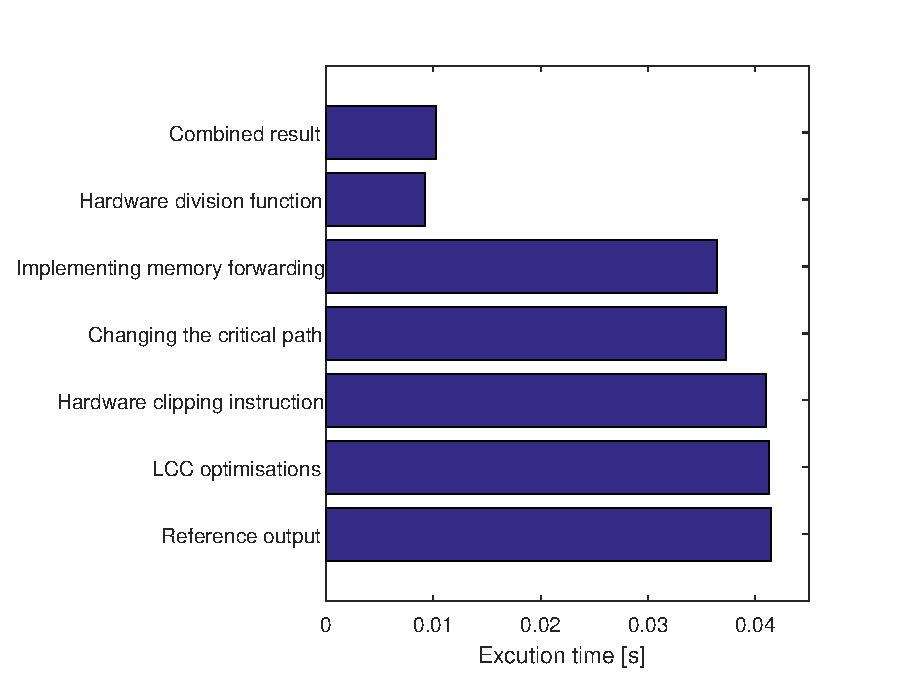
\includegraphics[height = 10cm]{image2.eps}
    \caption{Execution time per optimisation}
    \label{fig:ex}
\end{figure}


\section{Conclusion}
Although the standard mini-MIPS processor is relatively fast it can be clearly seen from the results in Table \ref{tab:speedimp} and Figure \ref{fig:ex} that large performance gains are possible to the mini-MIPS processor.\\
These large performance gains can even be further improved by implementing the remainder of optimisations that are listed in the optimisation list 1.\\ %is further improved and optimised.\\ 
Although there are different methods for optimising the processor, each with its own advantage and disadvantage the most notable performance gain can be achieved by implementing a hardware division instead of doing the division in software.\\
The performance gain that is achieved by a hardware division is tremendously large with a gain of 78\% .\\
While this gain is achieved with little extra cost for the hardware. The reason that such a large performance gain is possible is due the fact that the standard mini-MIPS processor uses software division and doing this division in hardware safes a lot of cycles.\\
The same can be said for many optimisations, the mini-MIPS processor can be greatly improved, at the cost of little extra hardware.\\
It can therefore be concluded that the RISC principle that the MIPS is based on makes the ISA of the MIPS fast,  yet large improvements can be made in order to further improve the number of cycles that need be to executed by the MIPS, this can mainly be done by better optimising the pipeline stages.

\section{References}

\begin{enumerate}

\item Retrieved March 15, 2016, from  \url{https://en.wikipedia.org/wiki/MIPS_instruction_set#Versions_of_the_MIPS_instruction_set }

\item Retrieved March 17, 2016, from \url{https://en.wikipedia.org/wiki/Moore%27s_law }

\item Retrieved March 18, 2016, from \url{https://en.wikipedia.org/wiki/SIMD }

\item Retrieved March 18, 2016, from \url{https://en.wikipedia.org/wiki/MIPS_instruction_set }

\item Retrieved March 20, 2016, from \url{https://en.wikipedia.org/wiki/Microcomputer_revolution }


\end{enumerate}


\end{document} 